\documentclass[12pt,parskip]{komatufte}
\usepackage[subpreambles=false]{standalone}

%%%%%%%%%%%%%%%%%%%%%%%%%%%
% Silence warning messages
\usepackage{silence}
\WarningsOff[scrlayer-notecolumn]
\WarningsOff[biblatex]

%%%%%%%%%%%%%%%%%%%%
% Commenting

%\usepackage[author=Lyndon]{pdfcomment}
%\newcommand{\pdfcomment}[1]{} %ignore all comments

%\usepackage{todonotes}
%\newcommand{\pdfcomment}{\todo}


%%%%%%%%%%%%%%%%%%%%
% Tables
\usepackage{booktabs}

%%%%%%%%%%%%%%%%%%%
% Fonts
\usepackage{tgadventor} %sans
\usepackage{tgpagella}  %serif
\usepackage{inconsolata} %mono
\usepackage[T1]{fontenc}

\usepackage{microtype}
\usepackage[all]{nowidow}
%%%%%%%%%%%%%%%%%%%%%%%
% Styling
\setcounter{secnumdepth}{4}
\setcounter{tocdepth}{2}

\usepackage{placeins}



%%%%%%%%%%%%%%%%%%%
% Math
\usepackage{amsmath, amssymb, stmaryrd, mathtools}
\DeclareMathOperator*{\argmin}{argmin}
\DeclareMathOperator*{\argmax}{argmax}

\usepackage{xparse,xstring,etoolbox}
% crossref this against notation section
\newcommand{\vv}[1]{\tilde{#1}} % vector
\newcommand{\seq}[1]{\mathcal{#1}} % sequence
\newcommand{\set}[1]{\mathbb{#1}} % set

%%%%%%%%%
% Indexing/sequence indexing
\newcommand{\seqind}[2]{#1^{#2}} % seqence index
\newcommand{\ind}[2]{#1_{#2}} % indexed
\newcommand{\disamb}[2]{#1^{\mathrm{#2}}} %disambiguated

%% Smart indexing and naming
\newcommand{\ifupper}[3]{
    \normalexpandarg
	\exploregroups
	\StrCount{ABCDEFGHIJKLMNOPQRSTUVWXYZ}{#1}[\uppercount]
	\ifnumgreater{\uppercount}{0}{#2}{#3}
}

%smart index
\DeclareDocumentCommand{\ii}{u{_} m}{
	\ifupper{#1}%
	{% just a single uppercase character, i.e. a matrix
		  %make sure the index is the right length
		\StrCount{#2}{,}[\indcount]
		\ifnumgreater{\indcount}{0}
		{ % Got multiple indexes so all good
		 	\ind{#1}{#2}
		}
		{ % Only 1 index so grab the column
		 	\ind{#1}{{:,#2}}
		}
	}%
	{% Not just a single upper case character
		\ind{#1}{#2}
	}
}

\DeclareDocumentCommand{\nn}{u{_} m}{
	\seqind{#1}{#2}
}

\DeclareDocumentCommand{\dd}{u{_} m}{
	\disamb{#1}{#2}
}

% Index of a vector
\DeclareDocumentCommand{\iv}{u{_} m}{\ii{\vv #1}_{#2}}
\DeclareDocumentCommand{\dv}{u{_} m}{\dd{\vv #1}_{#2}}
\DeclareDocumentCommand{\nv}{u{_} m}{\nn{\vv #1}_{#2}}

%exp
\let\oldexp\exp
\renewcommand{\exp}[1]{\oldexp \left( #1 \right)}
\newcommand{\exptwo}[1]{\oldexp_2 \left( #1 \right)}

\newcommand{\softmax}{\mathrm{smax}}

\DeclareMathOperator*{\expectedop}{\mathbb{E}}
\DeclareDocumentCommand{\expected}{u{_} m}{
	\expectedop\limits_{\mathrlap{#2}}
}

%%%%%%%%%%%%%%%%
%Graphics
\usepackage{tikz}
\usetikzlibrary{positioning, fit,  shapes.geometric}
\usepackage{ifthen}
\usepackage{etoolbox}

\tikzset{
	backgroundcolor/.style ={fill=white},
	every node/.append style={
		minimum height=7mm,
	},
	labe/.append style={
		%Blue,
		align = center,
		backgroundcolor,
		fill opacity=0.6,
		text opacity=1,
		font={\footnotesize\itshape}	
	},
	layer/.append style={
		draw,
		align = center,
		minimum height=7mm,
	},
	tight/.append style={
		inner sep=0.2mm,
	},
	lookupbox/.append style={
		draw=none,
		append after command={
		       	[shorten <= -0.5\pgflinewidth]
		       	([shift={(-1.5\pgflinewidth,-0.5\pgflinewidth)}]\tikzlastnode.north east)
		       	edge([shift={( 0.5\pgflinewidth,-0.5\pgflinewidth)}]\tikzlastnode.north west) 
		       	([shift={( 0.5\pgflinewidth,-0.5\pgflinewidth)}]\tikzlastnode.north west)
		       	edge([shift={( 0.5\pgflinewidth,-1.5\pgflinewidth)}]\tikzlastnode.south west)            
		       	([shift={( -1.5\pgflinewidth,+0.5\pgflinewidth)}]\tikzlastnode.south east)
		       	edge([shift={(-1.5\pgflinewidth,-0.5\pgflinewidth)}]\tikzlastnode.north east)
		},
		inner sep=0.7mm,
		outer sep=0mm,
		minimum width=25mm
	}
}

\usepackage{pgfplots}
\pgfplotsset{compat=1.14}
\pgfplotsset{sideplot/.append style={
		width=\notescolwidth,
		domain=-10:10,
		samples=101,
		smooth,
		enlarge y limits={abs=2},
		axis lines=middle,
		xlabel  = $z$,
		ylabel  = $y$,
	},
	equ/.append style={
		color=blue,
		thick,
		mark=none
	}
}

% Function  For a plot 
% it  needs to be declared in preamble because of how \makenote* interacts with multiple files
\def\errorsurface(#1,#2){(0.5*#1 + 0.7*#2 + sin(deg(1.5*#1 + #2^2)))^2}


\usepackage{graphicx}
\graphicspath{{./figs/}, {./}, {./figs/chaptersentencerrepr/}, {./figs/chapterintromachinelearning/}, {./figs/chapterwordrepr/}}
\usepackage{adjustbox}


%%%%%%%%%%%%%%%%%%%
% Refs
\usepackage{cleveref}

\addbibresource{master.bib}

%%%%%%%%%%%%%%%%%%%%
% Formatting

% for examples from natural language space.
\newcommand{\natlang}[1]{\ifmmode \text{``\texttt{#1}''} \else {``\texttt{#1}''}\fi}
% \ifmmode ``trick'' from https://tex.stackexchange.com/a/15194/5834

%%%%%%%%%%%%%%%%%%%%%



\begin{document}

\setchapterpreamble{%
	\dictum[\textit{English Composition and Literature}, Webster, 1923]
	{
		A sentence is a group of words expressing a complete thought.
	}
}
\chapter{Sentence Representations and Beyond}\label{sec:sentence-representations-and-beyond}
\begin{abstract}
	Chapter 8: Sentence representations and beyond (5-10 pages)
	This chapter takes the previous discussion of phrases to the next level: sentences.
	This will include discussions of works on recursive structure
	As well work leveraging recurrent neural networks.
	Methods that do not strongly consider order (including Sum of Word Embeddings; paragraph vectors) will also be discussed here.
	Many of these techniques extent to arbitrary length sequences of words.
\end{abstract}

\aside[Documents vs Sentences]{All techniques which can represent documents (or paragraphs) can by necessity represent sentences as well. A single sentence can be a whole document. Similarly for paragraphs. The reverse is not necessarily true.}


It can be argued that the core of true AI,
is the capture a machine manipulatable representation of an idea.
In natural language a sentence (as defined by Webster in the quote above),
is such a representation of an idea, but it is not machine manipulatable.
As such the conversion of sentences to a machine manipulatable representation is an important task in AI research.

\aside[Word Sense Embeddings as a by-product]{
Almost all sentence representation methods product word embeddings as a by-product
Either output embeddings, from softmax,
or input embeddings that are used as the networks inputs.}
\aside[Initialising input embeddings]{
In the case of systems with input embeddings it is common (but not ubiquitous) to initialised them using a pretrained embeddings from one of the methods discussed in the \Cref{sec:word-representations},
then allow them to be fine-tuned while training the sentence embeddings.
}

\section{Unordered and Weakly Ordered Representations}

\subsection{Sums of Word Embeddings}
\aside[SOWE is a BOW product]{
	The reader may recall from \Cref{sec:word-representations},
	that a word-embedding lookup is the same as a one-hot vector product:
	$C_{w_i} = C\,\hat{e}_{w_i}$.
	Similar can be said for sum of word embeddings (SOWE) and bag of words (BOW).
	For some set of words $\mathcal{W} = \lbrace{w_1,\ldots, w_n}$:
	the BOW representation is $B_\mathcal{W} = \sum_{w_i\in \mathcal{W}} \hat{e}_{w_i}$;
	the SOWE representation is $\sum_{w_i\in \mathcal{W}} C_{w_i} = CB_\mathcal{W}$.
	As with word-embeddings it is immensely cheaper to calculate this via lookup, than via matrix product;
	except on systems with suitable sparse matrix product tricks.	
}

Classically in information retrieval documents have been represented by bags of words (BOW).
That is to say a vector with length equal to the size of the vocabulary, with each position representing the count of the number of occurrences of a single word.
This is much the same as a one-hot vector representing a word, but with every word in the sentence/document counted.
The word embedding equivalent is sums of word embeddings (SOWE), and means of word embeddings (MOWE).
These methods, like BOW, lose all order information in the representation.
In many cases it is possible to recover a BOW from a much lower dimensional SOWE 

Surprisingly, they have been found on many tasks to be extremely well performing, better than several of the more advanced techniques discussed later in this chapter  \pcite{White2015SentVecMeaning}, \pcite{RitterPosition}.
It has been suggested that this is because in English there are only a few likely ways to order any given bag of words and thus original sentences can often be recovered from BOW \pcite{Horvat2014} and thus SOWE, \pcite{White2016a}, given a simple ngram language model.
The step beyond this is to encode the ngrams into a bag of words like structure.
The bag of ngrams (BON), e.g. bag of trigrams, has been classically used as an alternative to BOW.
Each index in the vector thus represents the occurrence of a ngram in the text.
So \natlang{It is a good day today}, has the 3grams: \natlang{(It is a)},\natlang{(is a good)},\natlang{(a good day)}, \natlang{(good day today)}.
As is obvious for all but the most pathological sentences, recovering the full sentence order from a bag of ngrams is possible even without a language model.

The natural analogy to this with word embeddings might seem to be to find ngram embeddings by the concatenation of $n$ word embeddings; and then to sum these.
However, such a sum is less informative than it might seem.
As the sum in each concatenated section is equal to the others, minus the edge words. To illustrate the case of trigram sums of word embeddings, for \natlang{It is a good day today},
the sums in each position would be:
\begin{align}
\left[\begin{array}{c|c|c}
	\sum & \sum & \sum\\
	C_{it} & C_{was} & C_{a}\\
	C_{was} & C_{a} & C_{good}\\
	C_{a} & C_{good} & C_{day}\\
	C_{good} & C_{day} & C_{today}
\end{array}\right]=\left[\begin{array}{c|c|c}
	C_{M}+C_{it}-C_{day} & C_{M} & C_{M}-C_{was}+C_{today}\end{array}\right]
\end{align}
\begin{align}
\left[\begin{array}{c|c|c}
	\quad C_{w_{1}} & \quad C_{w_{2}} & \quad C_{w_{3}}\\
	+C_{w_{2}} & +C_{w_{3}} & +C_{w_{4}}\\
	+C_{w_{3}} & +C_{w_{4}} & +C_{w_{5}}\\
	+C_{w_{4}} & +C_{w_{5}} & +C_{w_{6}}
\end{array}\right]=\left[\begin{array}{c|c|c}
	\sum C_{w_{i}}-C_{w_{n-1}}-C_{w_{n-2}} & \sum C_{w_{i}}-C_{w_{1}}-C_{w_{n-1}} & \sum C_{w_{i}}-C_{w_{1}}-C_{w_{2}}\end{array}\right]
\end{align}


\section{Sequential Models}

\begin{figure}
	\caption{The unrolled structure of an RNN for us in Encoding, Decoding and Encoding-Decoding (sequence-to-sequence) problems. RU is the recurrent unit -- the neural network which reoccurs at each time step. (Repeated from \Cref{fig-rnns})
	}
	
	\label{fig-rnns-sq}
	
	\resizebox{\textwidth}{!}{\documentclass[landscape]{article}
\usepackage[a3paper]{geometry}

\usepackage{tikz}
\usetikzlibrary{positioning, fit,  shapes.geometric}
\usepackage{ifthen}
\usepackage{etoolbox}

\tikzset{
	backgroundcolor/.style ={fill=white},
	every node/.append style={
		minimum height=7mm,
	},
	labe/.append style={
		%Blue,
		align = center,
		backgroundcolor,
		fill opacity=0.6,
		text opacity=1,
		font={\footnotesize\itshape}	
	},
	layer/.append style={
		draw,
		align = center,
		minimum height=7mm,
	},
	tight/.append style={
		inner sep=0.2mm,
	},
	lookupbox/.append style={
		draw=none,
		append after command={
		       	[shorten <= -0.5\pgflinewidth]
		       	([shift={(-1.5\pgflinewidth,-0.5\pgflinewidth)}]\tikzlastnode.north east)
		       	edge([shift={( 0.5\pgflinewidth,-0.5\pgflinewidth)}]\tikzlastnode.north west) 
		       	([shift={( 0.5\pgflinewidth,-0.5\pgflinewidth)}]\tikzlastnode.north west)
		       	edge([shift={( 0.5\pgflinewidth,-1.5\pgflinewidth)}]\tikzlastnode.south west)            
		       	([shift={( -1.5\pgflinewidth,+0.5\pgflinewidth)}]\tikzlastnode.south east)
		       	edge([shift={(-1.5\pgflinewidth,-0.5\pgflinewidth)}]\tikzlastnode.north east)
		},
		inner sep=0.7mm,
		outer sep=0mm,
		minimum width=25mm
	}
}
\usepackage{amsmath, amssymb, stmaryrd, mathtools}
\DeclareMathOperator*{\argmin}{argmin}
\DeclareMathOperator*{\argmax}{argmax}

\usepackage{xparse,xstring,etoolbox}
% crossref this against notation section
\newcommand{\vv}[1]{\tilde{#1}} % vector
\newcommand{\seq}[1]{\mathcal{#1}} % sequence
\newcommand{\set}[1]{\mathbb{#1}} % set

%%%%%%%%%
% Indexing/sequence indexing
\newcommand{\seqind}[2]{#1^{#2}} % seqence index
\newcommand{\ind}[2]{#1_{#2}} % indexed
\newcommand{\disamb}[2]{#1^{\mathrm{#2}}} %disambiguated

%% Smart indexing and naming
\newcommand{\ifupper}[3]{
    \normalexpandarg
	\exploregroups
	\StrCount{ABCDEFGHIJKLMNOPQRSTUVWXYZ}{#1}[\uppercount]
	\ifnumgreater{\uppercount}{0}{#2}{#3}
}

%smart index
\DeclareDocumentCommand{\ii}{u{_} m}{
	\ifupper{#1}%
	{% just a single uppercase character, i.e. a matrix
		  %make sure the index is the right length
		\StrCount{#2}{,}[\indcount]
		\ifnumgreater{\indcount}{0}
		{ % Got multiple indexes so all good
		 	\ind{#1}{#2}
		}
		{ % Only 1 index so grab the column
		 	\ind{#1}{{:,#2}}
		}
	}%
	{% Not just a single upper case character
		\ind{#1}{#2}
	}
}

\DeclareDocumentCommand{\nn}{u{_} m}{
	\seqind{#1}{#2}
}

\DeclareDocumentCommand{\dd}{u{_} m}{
	\disamb{#1}{#2}
}

% Index of a vector
\DeclareDocumentCommand{\iv}{u{_} m}{\ii{\vv #1}_{#2}}
\DeclareDocumentCommand{\dv}{u{_} m}{\dd{\vv #1}_{#2}}
\DeclareDocumentCommand{\nv}{u{_} m}{\nn{\vv #1}_{#2}}

%exp
\let\oldexp\exp
\renewcommand{\exp}[1]{\oldexp \left( #1 \right)}
\newcommand{\exptwo}[1]{\oldexp_2 \left( #1 \right)}

\newcommand{\softmax}{\mathrm{smax}}

\DeclareMathOperator*{\expectedop}{\mathbb{E}}
\DeclareDocumentCommand{\expected}{u{_} m}{
	\expectedop\limits_{\mathrlap{#2}}
}

\begin{document}

\numdef{\N}{8}
\numdef{\labelwidth}{5.5cm}
%%%%%%%%%%%%%%%%%%%%%%%%%
% Encoder

\begin{tikzpicture}[]

\begin{scope}
	\node(lblEncoder)[text width= \labelwidth] {\textbf{RNN Encoder:}\\%
	Variable $n$ inputs: $\nv x_t$\\%
	1 output: $\hat{y}$ \\%
	};
	
	\coordinate (L0) at (lblEncoder.east);
	
	\foreach \I[count=\j from 0] in {1,...,\N}{
		\ifnumequal{\I}{\N - 1}{%
			\node(L\I)[dashed, layer, right = of L\j] {...};
			\node(w\I)[below = of L\I]{...};
		}%
		{	
			\node(L\I)[layer, right = of L\j] {RU};
			\node(w\I)[below = of L\I]{\ifnumequal{\I}{\N}{$\nv x_n$}{$\nv x_\I$}};
			\draw[->](w\I) -- (L\I);
		}
	}
	\foreach \I[count=\j from 1] in {2,...,\N} {
		\draw[->] (L\j) edge node[labe]{state} (L\I);
	}
	
	\node(out) [above = of L\N]{$\hat{y}$};
	\draw[->] (L\N) -- (out);
\end{scope}

%%%%%%%%%%%%%%%%
% Decoder
\begin{scope}[yshift=-5cm] 
\node(lbl)[text width= \labelwidth] {\textbf{RNN Decoder:}\\%
1 input: $x$\\%
variable $m$ outputs: $\n \hat{y}_t$ \\%
with prompts: $\nv r_t$ (often $\nv y_{t-1}$)
};

\coordinate (L0) at (lbl.east);
\coordinate (L1c)[right = of L0];
\node(x)[below right = 4 of L1c]{$x$};

\foreach \I[count=\j from 0] in {1,...,\N}{
	\ifnumequal{\I}{\N - 1}{%
		\node(L\I)[dashed, layer, right = of L\j] {...};
		\node(w\I)[above = of L\I]{...};
		\node(y\I)[below = of L\I]{...};
	}%
	{	
		\node(L\I)[layer, right = of L\j] {RU};
		\node(v\I)[above = of L\I]{\ifnumequal{\I}{\N}{$\n \hat{y}_m$}{$\n \hat{y}_\I$}};
		\node(w\I)[below = of L\I]{$[\nv r_\I; \v x]$};
		\draw[->](w\I) -- (L\I);
		\draw[->](L\I) -- (v\I);
		\draw[->](x) to[bend right = 5] (w\I.300);
	}
}
\foreach \I[count=\j from 1] in {2,...,\N} {
	\draw[->] (L\j) edge node[labe]{state} (L\I);
}

\end{scope}
%
%%%%%%%%%%%%%%%%%%
% Encoder Decoder
%
\begin{scope}[yshift=-14cm]
\node(lbl)[text width= \labelwidth] {\textbf{RNN Encoder-Decoder:}\\%
Variable $n$ inputs: $\nv x_t$\\%
Variable $m$ outputs $\n \hat{y}_t$\\%
Prompts: $\nv r_t$ (often $y_{t-1}$)
};

\coordinate (L0) at (lbl.east);
\numdef{\NN}{4}
\foreach \I[count=\j from 0] in {1,...,\NN}{
	\ifnumequal{\I}{\NN - 1}{%
		\node(L\I)[dashed, layer, right = of L\j] {...};
		\node(w\I)[below = of L\I]{...};
	}%
	{
		\node(L\I)[layer, right = of L\j] {$\mathrm{RU_E}$};
		\node(w\I)[below = of L\I]{\ifnumequal{\I}{\NN}{$\nv x_n$}{$\nv x_\I$}};
		\draw[->] (w\I) -- (L\I);
	}
}
\foreach \I[count=\j from 1] in {2,...,\NN} {
	\draw[->] (L\j) edge node[labe] {state} (L\I);
}




\coordinate[above = 3 of L\NN] (Lp\NN);
\numdef{\NP}{\N - 1}
\foreach \j in {\NN,...,\NP}{
	\numdef{\I}{\j+1}
	\numdef{\y}{\I - \NN}
	\ifnumequal{\I}{\N-1}{%
		\node(Lp\I)[dashed, layer, right = of Lp\j] {...};
		\node(w\I)[below = of Lp\I]{...};
		\node(y\I)[above = of Lp\I]{...};
	}%
	{
		\node(Lp\I)[layer, right = of Lp\j] {$\mathrm{RU_D}$};
		\ifnumequal{\I}{\N}{
			\node(w\I)[below = of Lp\I]{$[\v z; \nv r_m]$};
			\node(y\I)[above = of Lp\I]{$\n \hat{y}_m$};
		}
		{
			\node(w\I)[below = of Lp\I]{$[\v z; \nv r_\y]$};
			\node(y\I)[above = of Lp\I]{$\n \hat{y}_\y$};
		}

		\draw[->] (w\I) -- (Lp\I);
		\draw[->] (Lp\I) -- (y\I);
		\path[->] (L\NN.north) edge node[labe]{$\v z$} (w\I.south west);
	}
}


\numdef{\NNp1}{\NN + 1}
\foreach \I in {\NNp1,...,\NP} {
	\numdef{\j}{\I+1}
	\draw[->] (Lp\I) edge node[labe] {state} (Lp\j);
}
 

\end{scope}


\end{tikzpicture}




\end{document}}
\end{figure}

The majority of this section draw on the recurrent neural networks (RNN) as discussed in \Cref{sec:rnn}.
We can used RNN encoders and decoders (as shown in \Cref{fig-rnns-sq}) to generate representations of sequences by extracting a coding layer.
In one can take any RNN encoder,
and select the one of the hidden layers after the final recurrent unit (RU) that has processed the last word in the sentence.
Similarly for any RNN decoder, one can select any hidden layer before the first recurrent unit that begins to produce words.
For an RNN encoder-decoder, this means selecting the hidden layer from between.
As for example in \tcite{cho-EtAl:2014:EMNLP2014}.


\tcite{Bowman2015SmoothGeneration} presents an extension on this notion,
where in-between the encoder and the decode stages there is a variational autoencoder (VAE).
The variational autoencoder \pcite{2014VAE} an autoencoder that has been demonstrated to have very good properties in a number of machine learning applications.
Using the VAE it is hoped that a better representation can be found for the sequence of words in the input and output.

Bowman et. al. training there network as encoder-decoder for English.
The VAE is the hidden coding layer.
They found that short syntactically similar sentences were located near to each other according to this space.
Further the that, because it has a decoder, it can generate these nearby sentences.

\begin{figure}
	
	\numdef{\n}{6}
	\numdef{\labelwidth}{5.5cm}
	%%%%%%%%%%%%%%%%%%%%%%%%%
	% Encoder
	\resizebox{\textwidth}{!}{
	\begin{tikzpicture}[]
	\coordinate (L0) at (lbl.east);
	\numdef{\nn}{\n/2}
	\foreach \i[count=\j from 0] in {1,...,\nn}{
		\ifnumequal{\i}{\nn - 1}{%
			\node(L\i)[dashed, layer, right = of L\j] {...};
			\node(w\i)[below = of L\i]{...};
		}%
		{
			\node(L\i)[layer, right = of L\j] {$\mathrm{RU_E}$};
			\node(w\i)[below = of L\i]{\ifnumequal{\i}{\nn}{$w_n$}{$w_\i$}};
			\draw[->] (w\i) -- (L\i);
		}
	}
	
	\numdef{\nvae}{\nn+1}
	\node(L_\nvae)[above=of L\nn] {VAE};
	\numdef{\nd}{\nvae+1}
	
	\numdef{\np}{\nd - 1}
	\foreach \j in {\nvae,...,\np}{
		\numdef{\i}{\j+1}
		\numdef{\y}{\i - \nn}
		\ifnumequal{\i}{\n-1}{%
			\node(L\i)[dashed, layer, right = of L\j] {...};
			\node(w\i)[below = of L\i]{...};
			\node(y\i)[above = of L\i]{...};
		}%
		{
			\node(L\i)[layer, right = of L\j] {$\mathrm{RU_D}$};
			\ifnumequal{\i}{\n}{
				\node(w\i)[below = of L\i]{$r_n$};
				\node(y\i)[above = of L\i]{$\hat{y}_m$};
			}
			{
				\node(w\i)[below = of L\i]{$r_\y$};
				\node(y\i)[above = of L\i]{$\hat{y}_\y$};
			}
			
			\draw[->] (w\i) -- (L\i);
			\draw[->] (L\i) -- (y\i);		
		}
	}
	
	\foreach \i[count=\j from 1] in {2,...,\n} {
		\draw[->] (L\j) edge node[labe] {\ifnumequal{\j}{\nn}{\underline{output}}{state}} (L\i);
	}
	% 
	\end{tikzpicture}}
	
\end{figure}


\section{Structured Models}
\aside[Parsers]{There are many high-quality parsing libraries available.
	Of particular note is the Stanford parser, included in Core NLP.
	It has bindings in many languages, including Python via NLTK.
	It has an interactive web-demo at \url{http://corenlp.run/},
	which was used to produce \Cref{fig:consparse,fig:depparse}
}

A limitation of sequential models is information only flows in a sequence.
However, the actual structure of natural language is not so simple.
Linguists tend to break sentences down into a tree or graph structure.
This is referred to as parsing.
The two most common are constituency parse trees, and dependency parse trees.
Examples of each are shown in \Cref{fig:consparse,fig:depparse}
It is beyond the scope of this book to explain the precise meaning of these trees.
The essence is that that represent the structure of the sentence,
according to how linguists currently understand how sentences are processed by humans.
The constituency parse breaks the sentence down into parts such as noun phrase (NP) and verb phrase (VP),
which are in turn broken down into phrases, or (POS tagged) words.
The constituency parse is well thought-of as a hierarchical breakdown of a sentence into its parts.
Conversely, a dependency parse is better thought of as a set of binary relations between head-terms and there dependent terms.
These structures are well linguistically motivated, so it make sense to use them in the processing of natural language.

\begin{figure}
	\caption{A constituency parse tree for the sentence \natlang{This is a simple example of a parse tree}}
	\centering{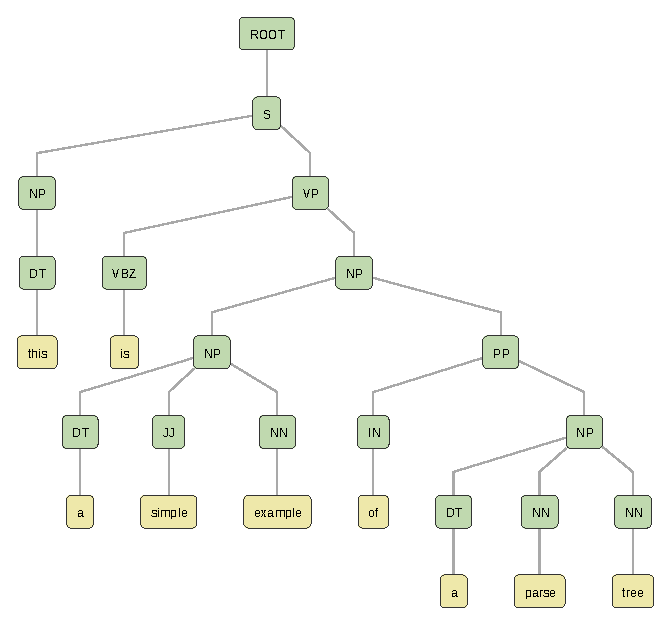
\includegraphics[width=\textwidth]{constparse}}
	\label{fig:consparse}
\end{figure}


\begin{figure}
	\caption{A dependency parse tree for the sentence \natlang{This is a simple example of a parse tree},
	This flattened view may be misleading.
	\natlang{example} is at the peak of the tree, with direct children	being:
	\natlang{this},\natlang{is},\natlang{a},\natlang{simple},
	and \natlang{tree}.
	\natlang{tree} has direct children being: \natlang{of},\natlang{a}, and \natlang{parse}.
}
	\centering{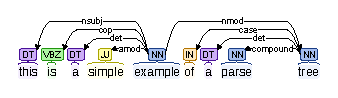
\includegraphics[width=\textwidth]{depparse}}
	\label{fig:depparse}
\end{figure}

We refer here to models incorporating tree, or graph structures as structural models.
Particular different variations have there own names, such as recursive neural networks (RvNN), and recurssive autoencoders (RAE).
We use the term structural model as an all encompassing term. 
It also makes for clearer reading to distinguish recursive and recurrent  neural networks.
Just as a linked list is but a particular case of a tree, an RNN is a particular case of a structural model,
however we will exclude them from this discussion except where marked.


The initial recent work on structural models was done in for the thesis of \tcite{socher2014recursive}.
It builds on the work of \tcite{goller1996BPstructure} and \tcite{Pollack199077}, which presents back-propagation through structure.
Back-propagation can be applied to networks of any structure, much like (and indeed directly because) the chain-rule can be applied to any equation to find its derivative.
This means that structuring a network according to its parse structure is possible.


These tree structured networks function apply an recursive unit (which we will call RV) across pairs (or other groups of) the representations of the lower levels, to produce a combined representation.

\begin{align}
	RV(u, v) &= \varphi\([S;R][u;v] + b \)\\
			 &= \varphi\(Su +Rv + b \)
\end{align}



\aside[Machine learning frameworks for structural models]{
Structural networks can not be defined in most modern static neural network frameworks,
such as TensorFlow.
These frameworks function by defining a single computational graph that is used to process each training/test case.
The same graph is used for each input.
By definition the structure of the network differs from training/test case to training/test case.
Technically the same problems apply to RNNs, as each case can have a different number of inputs.
This is normally worked around by defining the network graph for the longest input to be considered,
then padding all the inputs to this length.
Such is not possible with structured networks.
Other tricks are possible but are significantly more difficult.
The exception to this is of-course via dynamic components to the static frameworks
(which TensorFlow and other such frameworks certainly do have).
Even in a dynamic tool it remains a non-trivial task to implement these networks.
}


\aside[Implementing Back-propagation through structure]{
Back-propagation through structure is conceptually not significantly more complex than back propagation through time,
in practice a very difficult algorithm to get right.
In implementation it is very important to test for correctness using gradient checks, as it is easy to make a mistake and end-up with models that seem to work ok, but are actually crippled due to some mistake in the coding.
Unfolding recursive autoencoders are particularly difficult,
as the gradient must be propagated from all leaves.
And output interior nodes can not have there gradients calculated until the gradients of their children are calculated.
The solution to this is to process the gradients using a priority queue,
where the priority is set by the depth of the node.
Thus ensuring all children are processes before there parents.
}



A limitation of these structural models compared to the sequential RNNs,
is there lack of explicit gating on memory (e.g. as in GRU and LSTM).
Any given path down a tree can be looked at as like an RNN comprised only of basic recurrent units.
However, these paths are much shorter (being the logarithm of) than the full sequential length of the sentence,
which offsets the need for such gating.
Recall that the gating is to provide longer short term memory.


\aside[Sequential models are often preferred to structural models]{
Sequential (RNN) models are much more heavily researched than structural (RvNN) models.
They have better software libraries, and are easier to implement.
In theory it is possible for a sequential model (with sufficiently deep and wide RUs) effectively internalise the connections that a structural model would posses.
}




\end{document}